\documentclass[a4paper,10pt]{article}
\usepackage[frenchb]{babel}
\usepackage[utf8]{inputenc}
\usepackage[T1]{fontenc}
\usepackage{graphics}
\title{Rapport Comsol}
\author{Dubois Benoît et Vigné Adrien}
\date{10 Décembre 2018}
\usepackage{multicol}

\newenvironment{Figure}
  {\par\medskip\noindent\minipage{\linewidth}}
  {\endminipage\par\medskip}

\begin{document}

\maketitle

\begin{abstract}
    Abstract
\end{abstract}

\begin{multicols}{2}

\section*{Introduction}

\section{Théorie}
On s'intéresse ici à une microbalance à quartz donc à la résonance du quartz. On peut modéliser un quartz comme un ensemble série de résistance,bobine,condensateur et parallèle d'un condensateur (figure ) . On trouve à partir de ce modèle et des paramètres géométriques du cristal de quartz le lien entre la résonance et la masse du cristal notamment.
$$  $$

Dans cette étude de microbalance on considère que la masse rajoutée fais partie du cristal et influence donc directement sur la masse du cristal et donc sur la fréquence de résonance.




\section{Modélisation}

Afin de prévoir la réponse de notre microbalance nous l'avons modélisé sous \textsc{Comsol}. Nous avons cherché l'influence du rayon et de l'épaisseur des couches d'or et de titane dans la fréquence de résonance de la microbalance. 

On lance alors deux études paramétriques en faisant varier le rayon puis l'épaisseur. On prend un pas de $50 \mu m$ entre $400 \mu m$ et le rayon du wafer de silicium. Pour l'épaisseur on fait varier les épaisseurs d'or et de titane de sorte que la somme de leurs épaisseurs fassent toujours $1 \mu m$.

\subsection{Variation de rayon}

\begin{figure}
    \centering
    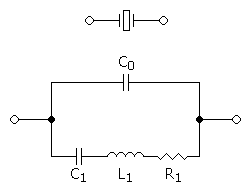
\includegraphics[width=\linewidth]{Quartz_crystal_equivalent.png}
    \captionof{Caption}
    \label{fig:my_label}
\end{figure}



\subsection{Variation d'épaisseur}




\section{Expériences}

\section{Résultats}

\section{Conclusion}


\end{multicols}
\end{document}
